\documentclass{beamer}
\usepackage[latin1]{inputenc}
\usepackage{xcolor}
\usepackage{hyperref}
\usepackage{minted}
\usepackage{tikz}
\usepackage{graphicx}
\usepackage{bbding} % For \HandRight
\usepackage{fancyvrb} % For \UseVerb \SaveVerb

\usetheme{Madrid}
\usecolortheme{default}

% Command that embeds a hand pointing to the right in a href label
\newcommand{\hrefhand}[2]{\raisebox{-0.4ex}{\HandRight}\,\href{#1}{#2}}

\title{COMP3320 Introduction to OpenGL}
\author{Alex Biddulph}
\institute{
    The University of Newcastle, Australia
    \and
    Based on the work provided at \url{www.learnopengl.com}
}
\date{Semester 2, 2021}

\begin{document}

\begin{frame}
    \titlepage
\end{frame}

\begin{frame}{OpenGL Coordinates}
    \begin{itemize}
        \item OpenGL uses a right-handed coordinate system
        \item OpenGL uses normalised device coordinates
        \item OpenGL will map the normalised device coordinates to the viewport dimensions
              \begin{itemize}
                  \item $\left(-1, -1\right) \to \left(0, 0\right)$
                  \item $\left(1, 1\right) \to \left(800, 600\right)$
              \end{itemize}
    \end{itemize}
    \begin{center}
        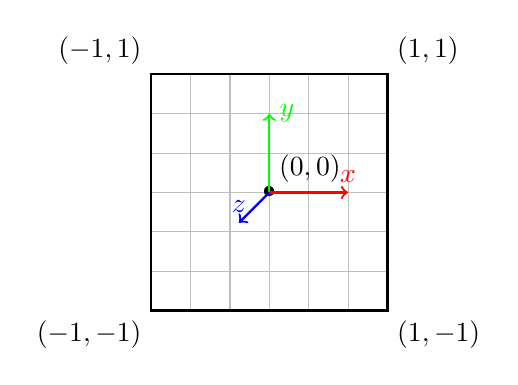
\begin{tikzpicture}[baseline={([yshift=-1em] current bounding box.north)}]
            % Grid lines
            \draw[step=0.5,lightgray,thin] (-1.5, -1.5) grid (1.5, 1.5);

            % Window edges
            \draw[thick] (-1.5, -1.5) -- (-1.5, 1.5) -- (1.5, 1.5) -- (1.5, -1.5) -- cycle;

            % Coordinates
            \draw (-1.5, -1.5) node[below left]{$\left(-1, -1\right)$};
            \draw (-1.5, 1.5) node[above left]{$\left(-1, 1\right)$};
            \draw (1.5, -1.5) node[below right]{$\left(1, -1\right)$};
            \draw (1.5, 1.5) node[above right]{$\left(1, 1\right)$};
            \draw (0, 0) node{\textbullet};
            \draw (0, 0) node[above right]{$\left(0, 0\right)$};

            % The axes
            \draw[thick,red,->]   (xyz cs:x=0.0) -- (xyz cs:x=1.0) node[above] {$x$};
            \draw[thick,green,->] (xyz cs:y=0.0) -- (xyz cs:y=1.0) node[right] {$y$};
            \draw[thick,blue,->]  (xyz cs:z=0.0) -- (xyz cs:z=1.0) node[above] {$z$};
        \end{tikzpicture}
    \end{center}
\end{frame}

\begin{frame}{OpenGL Coordinate Spaces}
    \begin{itemize}
        \item Local Space: 3D coordinates which are local to an object
        \item World Space: 3D coordinates within the world. The model matrix is used to transform coordinates from local space to world space
        \item View Space: Also known as camera space or eye space. View space is the camera's perspective of your world. The view matrix is used to transform coordinates from world space to view space
        \item Clip Space: A projection from view space to normalised device coordinates. The projection matrix is used to perform this projection. OpenGL expects the output of the vertex shader to be in clip space
    \end{itemize}
\end{frame}

\begin{frame}{OpenGL Shaders - Pipeline 1}
    \begin{itemize}
        \item Vertex Data: A list of 3D vertex coordinates and associated vertex attributes (we will come back to these later)
        \item Vertex Shader: Transforms vertex coordinates from model space to clip space
        \item Shape Assembly: Assembles transformed vertices into a given primitive shape (e.g. triangles)
        \item Geometry Shader: Transforms shape geometry by emitting new vertices
        \item Rasterization: Maps primitives to pixel space and creates fragments
        \item Fragment Shader: Calculates the final colour for a fragment
        \item Tests and Blending: Performs depth testing and alpha blending
    \end{itemize}
\end{frame}

\begin{frame}{OpenGL Shaders - Pipeline 2}
    \begin{figure}
        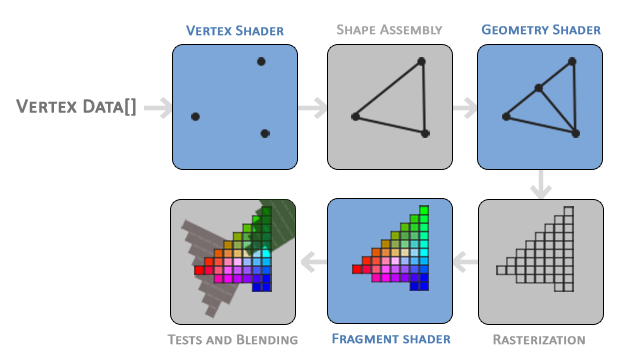
\includegraphics{images/pipeline.png}
        \caption{Graphics pipeline stages.}
    \end{figure}
    \vfill{}
    Image sourced from \url{learnopengl.com/Getting-started/Hello-Triangle}
\end{frame}

\begin{frame}[fragile]{OpenGL Shaders}
    \begin{itemize}
        \item Written in OpenGL Shader Language (GLSL)
        \item A simple vertex shader
              \begin{minted}{glsl}
#version 330 core
layout (location = 0) in vec3 aPosition;
void main() { gl_Position = vec4(aPosition, 1.0); }
\end{minted}
        \item A simple fragment shader
              \begin{minted}{glsl}
#version 330 core
layout (location = 0) out vec4 FragColour;
void main() {FragColour = vec4(1.0f, 0.5f, 0.2f, 1.0f);}
\end{minted}
    \end{itemize}
\end{frame}

\begin{frame}[fragile]{Useful Functions for Shaders}

    \SaveVerb{glCreateShader}|glCreateShader|
    \SaveVerb{glShaderSource}|glShaderSource|
    \SaveVerb{glCompileShader}|glCompileShader|
    \begin{examples}
        Create a shader using \hrefhand{https://www.khronos.org/registry/OpenGL-Refpages/gl4/html/glCreateShader.xhtml}{\color{blue}\UseVerb{glCreateShader}}
    \end{examples}
    \begin{examples}
        Attach shader source code using \hrefhand{https://www.khronos.org/registry/OpenGL-Refpages/gl4/html/glShaderSource.xhtml}{\color{blue}\UseVerb{glShaderSource}}
    \end{examples}
    \begin{examples}
        Compile a shader using \hrefhand{https://www.khronos.org/registry/OpenGL-Refpages/gl4/html/glCompileShader.xhtml}{\color{blue}\UseVerb{glCompileShader}}
    \end{examples}
\end{frame}

\begin{frame}[fragile]{OpenGL Shader Programs}
    \begin{itemize}
        \item Consists of multiple OpenGL shaders
              \begin{itemize}
                  \item If you have a vertex shader, you must have a fragment shader
                  \item If you have a fragment shader, you must have a vertex shader
                  \item Geometry shader is optional
              \end{itemize}
        \item \textbf{Vertex Shader:} Processes vertex data. Transforms model space coordinates to clip space coordinates
        \item \textbf{Geometry Shader:} Processes geometric primitive data. Modifies individual vertices in a primitive, either by moving the vertices or adding/deleting vertices
        \item \textbf{Fragment Shader:} Processes fragment data. Calculates lighting conditions for each fragment and assigns the final fragment colour
    \end{itemize}
\end{frame}

\begin{frame}[fragile]{Useful Functions for Shader Programs}

    \SaveVerb{glCreateProgram}|glCreateProgram|
    \SaveVerb{glAttachShader}|glAttachShader|
    \SaveVerb{glLinkProgram}|glLinkProgram|
    \SaveVerb{glUseProgram}|glUseProgram|
    \begin{examples}
        Create a shader program using \hrefhand{https://www.khronos.org/registry/OpenGL-Refpages/gl4/html/glCreateProgram.xhtml}{\color{blue}\UseVerb{glCreateProgram}}
    \end{examples}
    \begin{examples}
        Attach shaders to the program using \hrefhand{https://www.khronos.org/registry/OpenGL-Refpages/gl4/html/glAttachShader.xhtml}{\color{blue}\UseVerb{glAttachShader}}
    \end{examples}
    \begin{examples}
        Link attached shaders together into the final program using \hrefhand{https://www.khronos.org/registry/OpenGL-Refpages/gl4/html/glLinkProgram.xhtml}{\color{blue}\UseVerb{glLinkProgram}}
    \end{examples}
    \begin{examples}
        Make a shader program active by using \hrefhand{https://www.khronos.org/registry/OpenGL-Refpages/gl4/html/glUseProgram.xhtml}{\color{blue}\UseVerb{glUseProgram}}
    \end{examples}
\end{frame}

\begin{frame}[fragile]{Vertex Buffer Objects}
    \begin{itemize}
        \item Stores vertex data in GPU memory
        \item Program could consist of multiple different vertex buffers
        \item Vertex data is defined as a list of 3D coordinates
              \footnotesize{
                  \begin{minted}{c++}
    float vertices[] = {-0.5f, -0.5f, 0.0f,
                         0.5f, -0.5f, 0.0f,
                         0.0f,  0.5f, 0.0f };
 \end{minted}
              }
    \end{itemize}

    \SaveVerb{glGenBuffers}|glGenBuffers|
    \SaveVerb{glBindBuffer}|glBindBuffer|
    \SaveVerb{glBufferData}|glBufferData|
    \begin{examples}
        To create a vertex buffer use \hrefhand{https://www.khronos.org/registry/OpenGL-Refpages/gl4/html/glGenBuffers.xhtml}{\color{blue}\UseVerb{glGenBuffers}}
    \end{examples}
    \begin{examples}
        To make a vertex buffer active use \hrefhand{https://www.khronos.org/registry/OpenGL-Refpages/gl4/html/glBindBuffer.xhtml}{\color{blue}\UseVerb{glBindBuffer}}
    \end{examples}
    \begin{examples}
        To copy vertex data to GPU memory use \hrefhand{https://www.khronos.org/registry/OpenGL-Refpages/gl4/html/glBufferData.xhtml}{\color{blue}\UseVerb{glBufferData}}
    \end{examples}
\end{frame}

\begin{frame}[fragile]{Vertex Array Objects}
    \begin{itemize}
        \item Manages vertex buffer objects and vertex attributes
        \item Program could consist of multiple different vertex arrays
        \item Bind and configure vertex buffer objects after binding the vertex array
    \end{itemize}

    \SaveVerb{glGenVertexArrays}|glGenVertexArrays|
    \SaveVerb{glBindVertexArray}|glBindVertexArray|
    \SaveVerb{glDrawArrays}|glDrawArrays|
    \begin{examples}
        To create a vertex array use \hrefhand{https://www.khronos.org/registry/OpenGL-Refpages/gl4/html/glGenVertexArrays.xhtml}{\color{blue}\UseVerb{glGenVertexArrays}}
    \end{examples}
    \begin{examples}
        To make a vertex array active use \hrefhand{https://www.khronos.org/registry/OpenGL-Refpages/gl4/html/glBindVertexArray.xhtml}{\color{blue}\UseVerb{glBindVertexArray}}
    \end{examples}
    \begin{examples}
        To render a vertex array use \hrefhand{https://www.khronos.org/registry/OpenGL-Refpages/gl4/html/glDrawArrays.xhtml}{\color{blue}\UseVerb{glDrawArrays}} or some other OpenGL drawing command after binding it
    \end{examples}
\end{frame}

\begin{frame}[fragile]{Element Buffer Objects}
    \begin{itemize}
        \item Stores indexes into the list of vertex data
        \item Makes it easy to draw shapes which share vertices
              \begin{itemize}
                  \item An easy example is a square, which contains 2 triangles
                        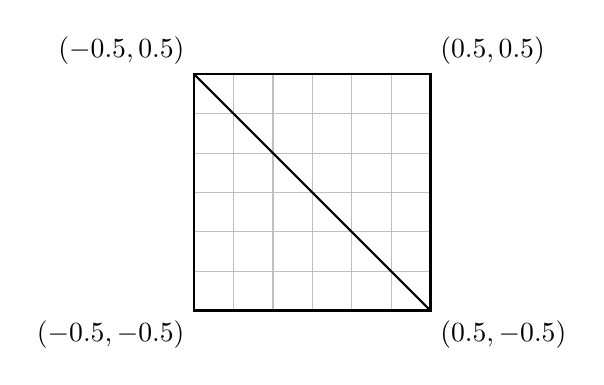
\begin{tikzpicture}[baseline={([yshift=-1em] current bounding box.north)}]
                            % Grid lines
                            \draw[step=0.5,lightgray,thin] (-1.5, -1.5) grid (1.5, 1.5);

                            % Window edges
                            \draw[thick] (-1.5, -1.5) -- (-1.5, 1.5) -- (1.5, 1.5) -- (1.5, -1.5) -- cycle;
                            \draw[thick] (-1.5, 1.5) -- (1.5, -1.5);

                            % Coordinates
                            \draw (-1.5, -1.5) node[below left]{$\left(-0.5, -0.5\right)$};
                            \draw (-1.5, 1.5) node[above left]{$\left(-0.5, 0.5\right)$};
                            \draw (1.5, 1.5) node[above right]{$\left(0.5, 0.5\right)$};
                            \draw (1.5, -1.5) node[below right]{$\left(0.5, -0.5\right)$};
                        \end{tikzpicture}
                  \item The naive way to draw this square would be to draw two triangles by specifying six vertices. Two of
                        the vertices would be repeated
                  \item The better way would be to list the four vertices in the square and use an element buffer object
              \end{itemize}
    \end{itemize}
\end{frame}

\begin{frame}[fragile]{Element Buffer Objects}
    \begin{itemize}
        \item Program could consist of multiple different element buffers
        \item Element data is defined as a list of integer indices
              \begin{minted}{c++}
    float vertices[] = {-0.5f, -0.5f, 0.0f,
                         0.5f, -0.5f, 0.0f,
                         0.5f,  0.5f, 0.0f,
                        -0.5f,  0.5f, 0.0f };
    unsigned int indices[] = {0, 1, 3,
                              1, 2, 3 };
 \end{minted}
        \item Vertex arrays will also track element buffers
    \end{itemize}
\end{frame}

\begin{frame}[fragile]{Usefule Functions for Element Buffer Objects}
    \SaveVerb{glGenBuffers}|glGenBuffers|
    \SaveVerb{glBindBuffer}|glBindBuffer|
    \SaveVerb{glBufferData}|glBufferData|
    \SaveVerb{glDrawElements}|glDrawElements|
    \begin{examples}
        To create an element buffer use \hrefhand{https://www.khronos.org/registry/OpenGL-Refpages/gl4/html/glGenBuffers.xhtml}{\color{blue}\UseVerb{glGenBuffers}}
    \end{examples}
    \begin{examples}
        To make an element buffer active use \hrefhand{https://www.khronos.org/registry/OpenGL-Refpages/gl4/html/glBindBuffer.xhtml}{\color{blue}\UseVerb{glBindBuffer}}
    \end{examples}
    \begin{examples}
        To copy index data to GPU memory use \hrefhand{https://www.khronos.org/registry/OpenGL-Refpages/gl4/html/glBufferData.xhtml}{\color{blue}\UseVerb{glBufferData}}
    \end{examples}
    \begin{examples}
        To render the data the data referenced by the element buffer use \hrefhand{https://www.khronos.org/registry/OpenGL-Refpages/gl4/html/glDrawElements.xhtml}{\color{blue}\UseVerb{glDrawElements}}
    \end{examples}
\end{frame}

\end{document}
